\documentclass[utf8, seminar, numeric]{fer}
\usepackage{booktabs}
\usepackage{hyperref}
\usepackage{siunitx}
\usepackage{amsmath}
\usepackage{placeins}
\usepackage{bm}

\begin{document}

\title{Analiza periodičkih struktura s naglaskom na fotoničke kristale
	   i izračun disperzijskog dijagrama}
\author{Darko Janeković}
\voditelj{dr.sc. Dario Bojanjac}

\maketitle

\tableofcontents


\chapter{Uvod}
U ovom seminaru bit će analizirane periodičke strukture s naglaskom na fotoničke
kristale primjenom numeričkih metoda za izračun disperzijskog dijagrama.
Programska biblioteka koja će se koristiti za numeričko modeliranje je
MPB(MIT Photonic Bands)\cite{Johnson2001:mpb}. Prije svega, bit će iznesena
matematička podloga potrebna za efikasno modeliranje propagacije vala u
periodičkoj strukturi. U poglavljima nakon uvoda bit će iznesena primjena
fotoničkih kristala, kao i numeričke metode korištene u svrhu modeliranja
problema koji opisuju periodičke strukture.


\chapter{Matematičko modeliranje propagacije vala u periodičkoj strukturi}

U ovom poglavlju nešto će detaljnije biti iznesena teorija periodičkih struktura
kao i matematički formalizam koji ih opisuje. Analiza propagacije vala unutar
periodičke rešetke prirodno navodi na Blochov teorem koji kaže da će polje u
periodičkoj strukturi poprimiti isti period i simetriju kao i period te strukture.
Kao polazišna točka, bit će izvedena valna jednadžba za propagaciju vala unutar
nehomogenog dielektrika. Svojstveni problem i njegova interpretacija bit će
razmatrani baš u okvirima te jednadžbe. Konačno će jednadžba pomoću Blochovog
teorema biti specijalizirana za slučaj fotoničkog kristala.


\section{Periodičke strukture i kristalna rešetka}

Periodička struktura je pravilna rešetkasta struktura u kojoj se elementi
periodički ponavljaju. Fotonički kristali su periodički strukturirani
elektromagnetski mediji koji generalno posjeduju svojstvo da svjetlost na
određenim frekvencijama ne propagira kroz strukturu. To svojstvo nazivat će se
fotonički frekvencijski raspor (engl. \textit{photonic band-gap}), a u nastavku
samo frekvencijski raspor. Fotonički kristali periodički su na način da
zadovoljavaju diskretnu translacijsku simetriju. Diskretnta translacijska
simetrija definirana je kao
${f(\mathbf{r}) = f(\mathbf{r} \pm \mathbf{a})}$, odnosno

\begin{equation}
	f(\mathbf{r}) = f(\mathbf{r} + \mathbf{R}) \text{, gdje je }{\mathbf{R} =
	n\mathbf{a}}, n \in \mathbb{Z}
\end{equation}

Vektor $\mathbf{a}$ naziva se osnovni vektor rešetke, a njegova duljina
naziva se konstanta rešetke, u nastavku samo $a$. Ćelija za koju se tvrdi
da svojim ponavljanjem tvori kristalnu rešetku naziva se jedinična ćelija.
Jedinična ćelija je najmanja jedinica kristalne rešetke koja svojim
ponavljanjem može tvoriti potpunu rešetku. Pored toga, ne postoji ćelija manjeg
volumena od ${|\mathbf{a}_1 \cdot \mathbf{a}_2 \times \mathbf{a}_3|}$, odnosno
volumena kojeg zatvaraju osnovni vektori rešetke.

\begin{figure}[ht]
	\centering
	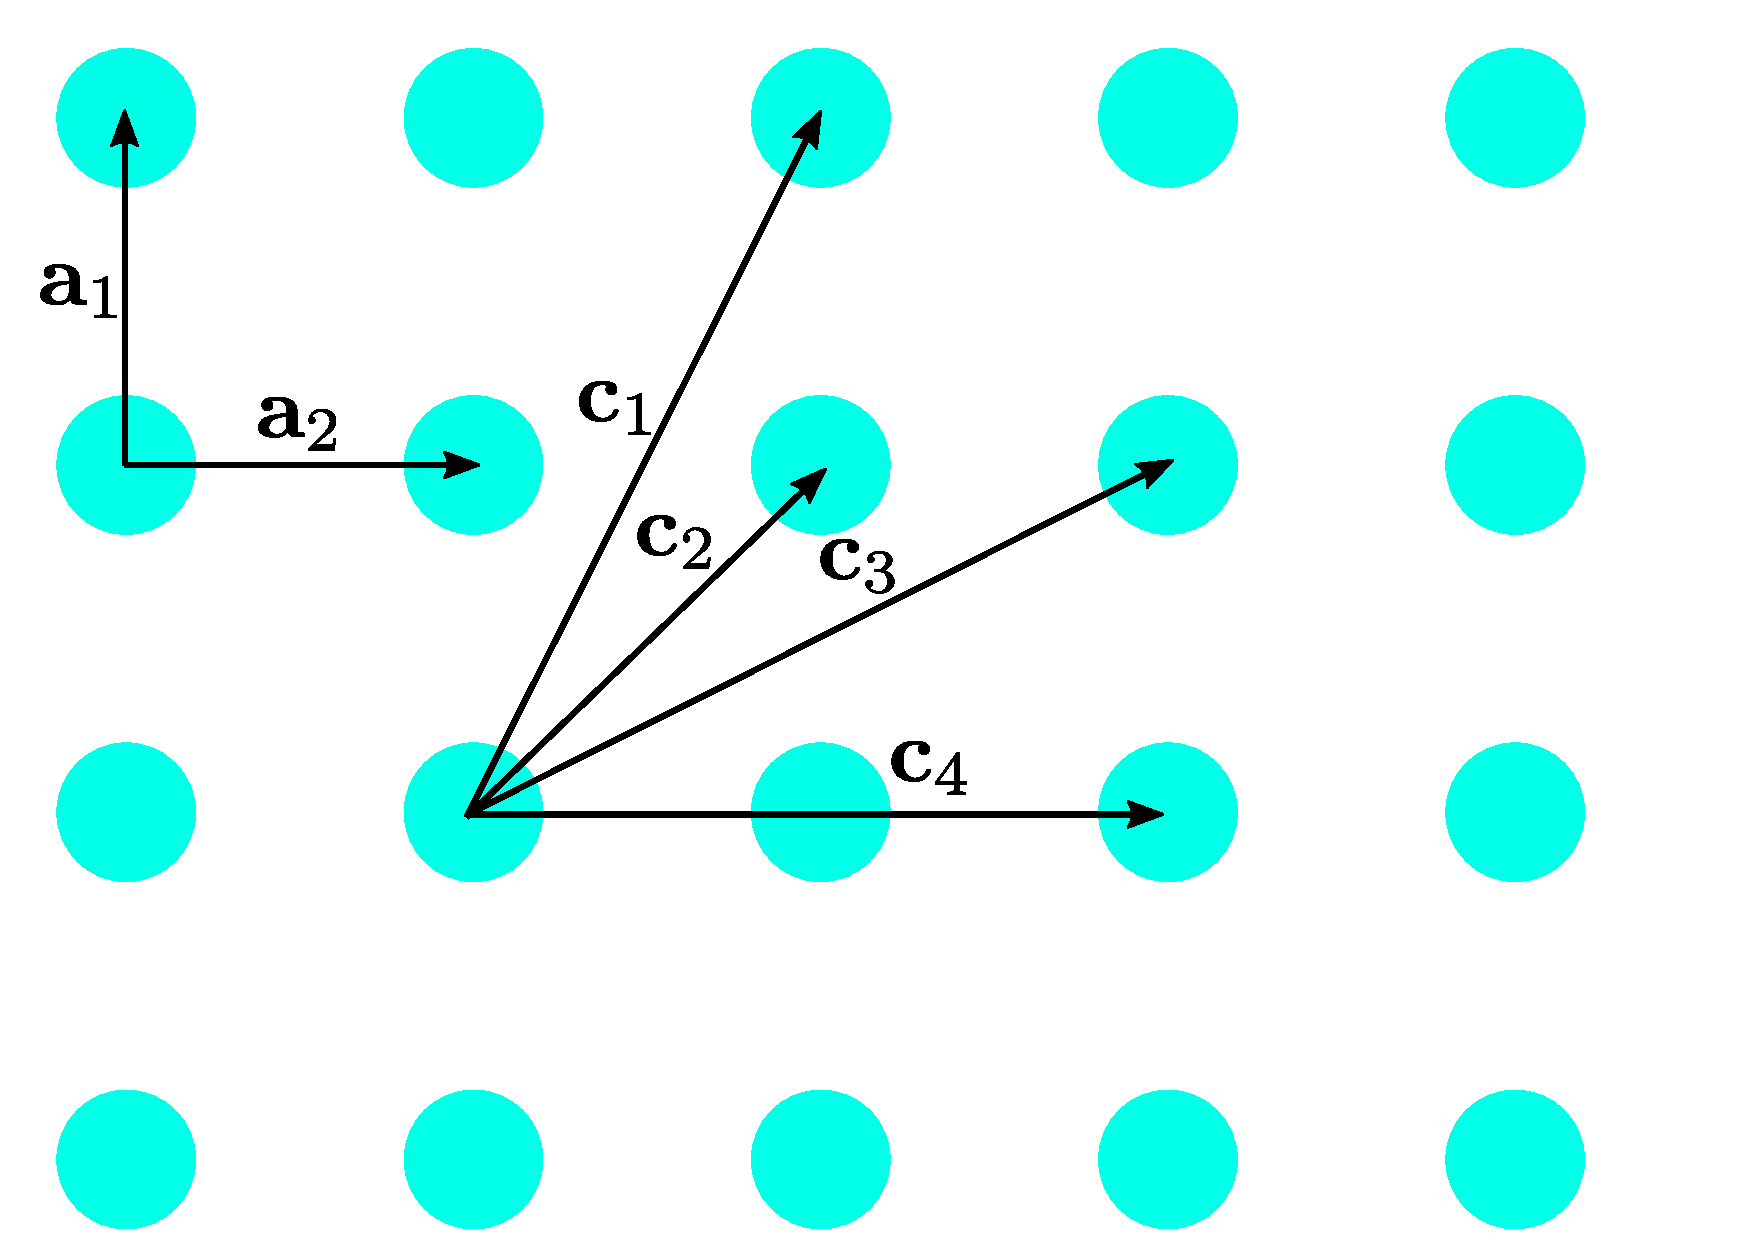
\includegraphics[width = 1.0\linewidth]{./images/crystal_lattice.pdf}
	\caption{Kvadratna kristalna rešetka s ucrtane 3 opcije za odabir baznih
	vektora $\mathbf{a}_1$ i $\mathbf{a}_2$. Linearna kombinacija vektora
	$\mathbf{a}_1 = a \, \mathbf{i}$ i $\mathbf{a}_2 = a \, \mathbf{j}$ (opcija
	pod a) tvori sve ostale vektore odnosno sva ostala čvorišta kristala.
	Konkretno,
	${\mathbf{c}_1 = \mathbf{a}_1 + 2 \, \mathbf{a}_2}$,
	${\mathbf{c}_2 = \mathbf{a}_1 + \mathbf{a}_2}$,
	${\mathbf{c}_3 = 2 \, \mathbf{a}_1 + \mathbf{a}_2}$,
	${\mathbf{c}_4 = 2 \, \mathbf{a}_1}$}
	\label{fig:crystal_lattice}
\end{figure}

Ovisno o dimenzionalnosti problema moguće je odabrati različite osnovne
vektore rešetke i sve ostale translacije prikazati kao linearnu kombinaciju
osnovnih vektora.

Weigner-Seintzova ćelija primjer je primitivne ćelije koja sadrži samo jedno
čvorište i predstavlja skup točaka u prostoru koji je bliži jednom čvorištu
od bilo kojeg drugog čvorišta. Čvorišta kristalne rešetke nalaze se u središtu
Weigner-Seintzove ćelije. Iako kristal ima beskonačno puno jediničnih ćelija,
on ima samo jednu Weigner-Seintzovu ćeliju.

Inverzna rešetka uvodi se za prikaz valnih vektora u Fourierovom razvoju
periodičnih funkcija. Vektori inverzne rešetke bit će označavani s $\mathbf{b}$.
Za vektore inverzne rešetke vrijedi:

\begin{equation}
	\mathbf{R} \cdot \mathbf{G} =
	(n_1\mathbf{a}_1 + n_2\mathbf{a}_2 + n_3\mathbf{a}_3)
	\cdot
	(m_1\mathbf{b}_1 + m_2\mathbf{b}_2 + m_3\mathbf{b}_3) = 2 \pi \mathbb{N},
		\text{ gdje je }n_i, m_i \in \mathbb{N}
\end{equation}


Weigner-Seintzova ćelija recipročne rešetke zove se Brillouinova zona. Analiza
disperzijskog dijagrama obavlja se u \textit{k prostoru}, prostoru recipročne
rešetke, odnosno u prvoj Brillouinovoj zoni. Ona označava najmanji
prostor unutar Brillouinove zone koji u potpunosti karakterizira polje unutar
periodičke strukture. Svaku točku unutar Brillouinove zone moguće je preslikati
% todo: istakni?
u prvu Brillouinovu zonu. Drugim riječima, analiza propagacije vala unutar
Brillouinove zone, bit će ekvivalentna analizi unutar prve Brillouinove zone uz
određenu redundantnost u računu. Što je rešetka više simetrična, to će biti
isplativije analizu obavljati unutar prve Brillouinove zone.


\section{Blochov teorem}

Intuitivnim razmišljanjem jasno je da će val koji je u jednom trenutku prolazio
kroz dielektrični objekt kasniti. Lako je onda generalizirati ideju na periodičku
strukturu i iz tog razmišljanja izvući zaključak da će polje unutar periodičke
strukture poprimiti isti period i simetriju kao i ta struktura. Teorem koji je
upravo intuitivno izveden naziva se Blochov teorem, i matematički formaliziran
glasi ovako:

\begin{equation} \label{eq:bloch}
	\mathbf{E}(\mathbf{r}) =
	\mathbf{A}_{\bm{\beta}}(\mathbf{r}) \cdot
		e^{j {\bm{\beta}} \cdot \mathbf{r}}
\end{equation}

U jednadžbi \ref{eq:bloch}, vektorsko polje $\mathbf{E}$ označava ukupno polje
u periodičkoj strukturi i ono se sastoji od dvije komponente. Vektorsko polje
$\mathbf{A}$ označava amplitudu s istim periodom i simetrijom kao i rešetka.
Ono diktira amplitudu ukupnog polja $\mathbf{E}$.
Komponenta ${e^{j {\bm{\beta}} \cdot \mathbf{r}}}$ označava ravni val i diktira
smjer propagacije vala.

% todo: ubaci meep sliku kako to izgleda i napiši par riječi o tome

% todo: matematički potkrijepi gore napisano + pročitaj više o ovome


\section{Izvod valne jednadžbe za propagaciju u sredstvu s nehomogenim dielektrikom}

U ovom potpoglavlju bit će izvedena valna jednadžba koja opisuje propagaciju
vala u nehomogenom dielektriku. Sredstvo u kojem val propagira nalikuje sredstvu
na slici \ref{fig:structure}.

\begin{figure}[ht]
	\centering
	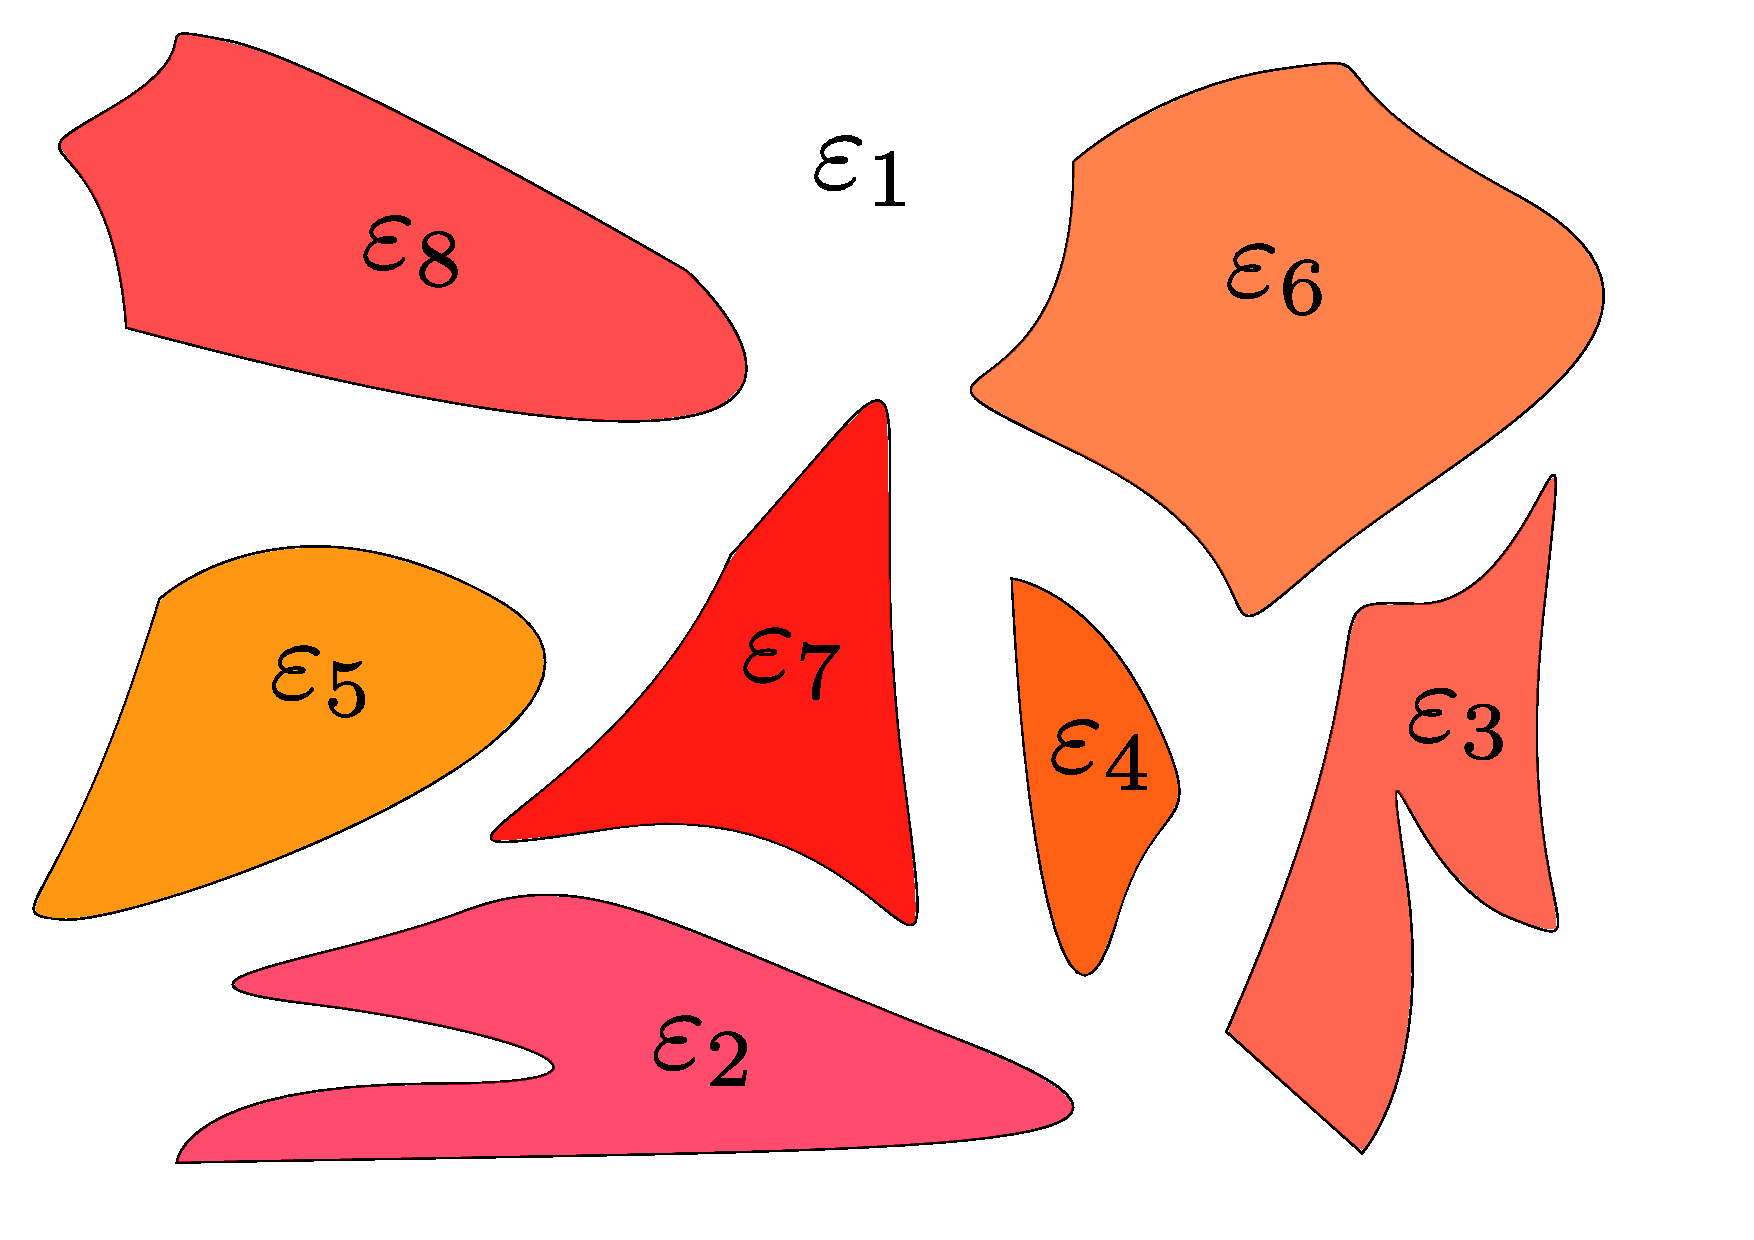
\includegraphics[width = 1.0\linewidth]{./images/structure-model.pdf}
	\caption{Model strukture u kojoj propagira val. Sredstvo je sastavljeno od
	neperiodičnih, homogenih poddomena različitih dielektričnih materijala.
	Poddomene se nalaze u materijalu permitivnosti $\varepsilon_1$.}
	\label{fig:structure}
\end{figure}

\FloatBarrier

Izvod valne jednadžbe, kao i za slučaj propagacije u homogenom sredstvu započinje
Maxwellovim jednadžbama:

\begin{align} \label{eq:maxwell1}
	\nabla \cdot \mathbf{D} = \rho &&
	\nabla \times \mathbf{E} &=
		- \frac{\partial \mathbf{B}}{\partial t}  \nonumber \\
	\nabla \cdot \mathbf{B} = 0 &&
	\nabla \times \mathbf{H} &=
		\mathbf{J} + \frac{\partial \mathbf{D}}{\partial t}
\end{align}

Permitivnost $\varepsilon$ u sredstvu postaje funkcija koja ovisi o položaju,
odnosno $\varepsilon(\mathbf{r})$. Pored toga, pretpostavlja se da struktura ne
mijenja konfiguraciju u vremenu te da u njoj nema izvora svjetlosti. Između
ostalog, pretpostavlja se da su snage dovoljno male kako bi sustav imalo smisla
promatrati u linearnom režimu. Materijali koji će se analizirati bit će
izotropni, odnosno $\varepsilon_r$ će biti skalarna funkcija. Kod
anizotropnih materijala $\mathbf{D}$ i $\mathbf{E}$ nisu vezani s
$\varepsilon_0 \varepsilon_r$, već s dielektričnim tenzorom
$\varepsilon_0 \varepsilon_{ij}$. S obzirom na frekvencije na kojima će se
obavljati analiza, ima smisla pretpostaviti $\mu_r = 1$. Konačno, nakon svih
pretpostavki jednadžbe \ref{eq:maxwell1} poprimaju sljedeći oblik:

\begin{align} \label{eq:maxwell2}
	\nabla \cdot (\varepsilon_r(\mathbf{r}) \mathbf{E}(\mathbf{r}, t)) = 0 &&
	\nabla \times \mathbf{E}(\mathbf{r}, t) &=
		- \mu_0
		\frac{\partial \mathbf{H}(\mathbf{r}, t)}{\partial t}  \nonumber \\
	\nabla \cdot \mathbf{H}(\mathbf{r}, t) = 0 &&
	\nabla \times \mathbf{H}(\mathbf{r}, t) &=
		\varepsilon_0 \varepsilon_r(\mathbf{r}, t)
		\frac{\partial \mathbf{E}(\mathbf{r}, t)}{\partial t}
\end{align}

Budući da su Maxwellove jednadžbe linearne, moguće je pretpostaviti da će odziv
titrati istom frekvencijom kao i pobuda. To svojstvo omogućava rastav polja
na prostornu i vremensku komponentu:
% TODO: napiši i pročitaj više o ovome
\begin{equation} \label{eq:harmonic}
	\mathbf{H}(\mathbf{r}, t) = \mathbf{H}(\mathbf{r}) e^{-i \omega t}
\end{equation}

Nakon uvrštavanja \ref{eq:harmonic} Maxwellove jednadžbe poprimaju sljedeći
oblik:

\begin{align} \label{eq:maxwell3}
	\nabla \cdot (\varepsilon_r(\mathbf{r}) \mathbf{E}(\mathbf{r})) = 0 &&
	\nabla \times \mathbf{E}(\mathbf{r}) &=
		i \omega \mu_0 \mu(\mathbf{r})\mathbf{H}(\mathbf{r})  \nonumber \\
	\nabla \cdot \mathbf{H}(\mathbf{r}) = 0 &&
	\nabla \times \mathbf{H}(\mathbf{r}) &=
		- i \omega \varepsilon_0 \varepsilon_r(\mathbf{r})\mathbf{E}(\mathbf{r})
\end{align}

Djelujući operatorom rotora na Faradayev zakon dobije se valna jednadžba u
sljedećem obliku:

\begin{equation} \label{eq:master}
	\nabla \times \left(\frac{1}{\varepsilon_r(\mathbf{r})}\nabla
			\times \mathbf{H}(\mathbf{r}) \right)
	= \left( \frac{\omega}{c} \right)^2 \mathbf{H}(\mathbf{r})
\end{equation}

Jednadžba \ref{eq:master} predstavljat će jednadžbu koja će biti korištena za
računanje disperzijskog dijagrama u nehomogenom dielektriku.
Ako se operator ${\nabla \times \frac{1}{\varepsilon_r(\mathbf{r})} \nabla \times}$
zamijeni s $\hat{\mathbf{\Theta}}$ dobiva se uobičajena forma svojstvenog
problema.

\begin{equation}
	\hat{\mathbf{\Theta}} \mathbf{H}(\mathbf{r}) =
		\left( \frac{\omega}{c} \right)^2 \mathbf{H}(\mathbf{r})
\end{equation}

Budući da je operator $\hat{\mathbf{\Theta}}$ hermitski
\footnote{
	Potrebno je dokazati da je ${(\mathbf{F}, \hat{\mathbf{\Theta}}\mathbf{G})
	=(\hat{\mathbf{\Theta}} \mathbf{F}, \mathbf{G})}$.

	$$(\mathbf{F}, \hat{\mathbf{\Theta}}\mathbf{G}) =
	\iiint \mathbf{F}^* (\mathbf{r}) \cdot \nabla \times \left(
		\frac{1}{\varepsilon_r (\mathbf{r})} \nabla \times \mathbf{G}(\mathbf{r})
	\right) \, \mathrm{d}^3 \mathbf{r}$$

	% dario citat
	Koristeći formulu za parcijalnu integraciju operacije rotora i Gaussov
	teorem izraz se svodi na

	%todo: ako će ti se dati ubaci oiint umjesto oint

	$$(\mathbf{F}, \hat{\mathbf{\Theta}}\mathbf{G}) =
	\iiint \frac{1}{\varepsilon_r (\mathbf{r})} \nabla \times \mathbf{G}(\mathbf{r})
	\cdot \left(
		\nabla \times \mathbf{F}(\mathbf{r})
	\right)^* \, \mathrm{d}^3 \mathbf{r}
	- \oint \left(
		\mathbf{F}^*(\mathbf{r}) \times \frac{1}{\varepsilon_r(\mathbf{r})}
		\nabla \times \mathbf{G}(\mathbf{r})
	\right) \hat{n} \, \mathrm{d}S$$

	Drugi član izraza zanemaruje se ili zbog periodičnosti na području integracije
	% todo: napiši ovo bolje: field decay to zero at large distances
	ili zato što polja teže u 0 pri velikim udaljenostima. Parcijalna integracija
	provodi se još jednom uz zanemarivanje istog člana kao i ranije.

	$$(\mathbf{F}, \hat{\mathbf{\Theta}}\mathbf{G}) =
	\iiint \mathbf{G}(\mathbf{r})
	\cdot \left[
		\nabla \times \left(
			\frac{1}{\varepsilon_r (\mathbf{r})} \nabla \times
			\mathbf{F}(\mathbf{r})
		\right)
	\right]^* \, \mathrm{d}^3 \mathbf{r}
	- \oint \left[
		\left(
			\frac{1}{\varepsilon_r(\mathbf{r})} \times \mathbf{F}(\mathbf{r})
		\right)^*
		\times \mathbf{G}(\mathbf{r})
	\right] \hat{n} \, \mathrm{d}S
	= (\hat{\mathbf{\Theta}} \mathbf{F}, \mathbf{G})$$
},
moguće je analizirati njegov Rayleighov kvocijent
$R \left(\hat{\mathbf{\Theta}}, \mathbf{H}(\mathbf{r}) \right)$.

Nadalje, može se pokazati da će najmanja svojstvena vrijednost $\omega_0^2/c^2$,
odnosno prvo nađeno rješenje svojstvenog problema minimizirati Rayleighov
kvocijent.

%TODO: Mislim da je ovo čudan rezultat i treba ga provjeriti ...
\begin{align}
	R \left( \hat{\mathbf{\Theta}}, \mathbf{H}(\mathbf{r}) \right)
	&= \frac{
		\omega^2/c^2
		\left(
			\mathbf{H}(\mathbf{r}), \mathbf{H}(\mathbf{r})
		\right)
	}
	{
		\omega^2/c^2
		\left(
			\mathbf{H}(\mathbf{r}), \hat{\mathbf{\Theta}}\mathbf{H}(\mathbf{r})
		\right)
	}
	= \frac{
		\iiint |\nabla \times \mathbf{E}(\mathbf{r})|^2
		\, \mathrm{d}^3\mathbf{r}}
	{\iiint \varepsilon_r(\mathbf{r}) | \mathbf{E}( \mathbf{r} ) |^2
	\, \mathrm{d}^3\mathbf{r}} \label{eq:rayleighE}
\end{align}

Budući da se kvocijent može minimizirati tako da se maksimizira nazivnik, iz
izraza \ref{eq:rayleighE} može se zaključiti da će električno polje
``preferirati'' područja veće permitivnosti. Drugim riječima,
najsnažnija električna polja mogu se očekivati u područjima veće permitivnosti.


\section{Propagacija vala unutar periodičke strukture}

Koristeći rezultat \ref{eq:master} i uvrštavajući \ref{eq:bloch} umjesto
$\mathbf{H}(\mathbf{r})$ dobiva se diferencijalna jednadžba koja predstavlja
svojstveni problem propagacije vala unutar fotoničkog kristala odnosno
periodičke strukture.

\begin{align} \label{eq:master_bloch}
	\nabla \times
	\frac{1}{\varepsilon_r(\mathbf{r})} \nabla \times
	\mathbf{H}_{\bm{\beta}}(\mathbf{r}) \cdot
	e^{j {\bm{\beta}} \cdot \mathbf{r}}
	= \left(
		\frac{\omega}{c}
	\right)^2
	\mathbf{H}_{\bm{\beta}}(\mathbf{r}) \cdot
		e^{j {\bm{\beta}} \cdot \mathbf{r}}	\nonumber \\
	(\nabla + j{\bm{\beta}}) \times
	\frac{1}{\varepsilon_r(\mathbf{r})}
	(\nabla + j{\bm{\beta}}) \times
	\mathbf{H}_{\bm{\beta}}(\mathbf{r})
	= \left(
	\frac{\omega ({\bm{\beta}})}{c}
	\right)^2
	\mathbf{H}_{\bm{\beta}}(\mathbf{r})
\end{align}

Jednadžba \ref{eq:master_bloch} predstavlja završnu jednadžbu koja služi za
proračun disperzijskog dijagrama u fotoničkom kristalu. Svojstvena vrijednost
${\omega ({\bm{\beta}})}$ je kontinuirana funkcija
Ovaj oblik
svojstvenog problema rješava programska biblioteka MPB spomenuta ranije. Sva
svojstva izvedena ranije, vrijede i za gore izvedenu jednadžbu.


\chapter{Proračun disperzijskog dijagrama fotoničkih kristala}

Imenovanje komponenata polja u kristalu bit će u skladu s imenovanjem u
literaturi \cite{joannopoulos2011photonic}. Kratica \textbf{TE},
\textit{transverse-electric} označavat će mod kod kojeg ne postoji komponenta
električnog polja u smjeru širenja vala. Slično, kratica \textbf{TM},
\textit{transverse-magnetic} označavat će mod kod kojeg ne postoji komponenta
magnetskog polja u smjeru širenja vala.

U poglavljima koja slijede bit će proračunati i prikazani disperzijski dijagrami
osnovnih dvodimenzionalnih fotoničkih kristala. Za početak će na primjeru
jednodimenzionalnog kristala biti objašnjeno nastajanje frekvencijskog raspora, a
zatim će biti opisane konfiguracije koje osiguravaju frekvencijski raspor (engl.
\textit{band-gap}) za TM, potom za TE, a onda i za oboje, odnosno potpuni
frekvencijski raspor.

Što se tiče disperzijskih dijagrama u nastavku, vrijedit će određeni skup pravila
koji će biti primjenjiv na sve dijagrame. TE komponenta uvijek će biti prikazana
plavom bojom, a TM crvenom. Frekvencijski raspori uvijek će biti prikazivani kao
plavi, odnosno crveni pravokutnici. Os x označavat će iznos valnog vektora
${\bm{\beta}}$, a y, normaliziranu frekvenciju izraženu kao
${\omega a/ 2 \pi c}$. Što se tiče prikaza modela fotoničkih kristala,
dielektrično sredstvo uvijek će biti obojano, dok će zrak biti označen bijelom
bojom. U opisu grafa bit će naznačeno s kojim je dimenzijama modeliran objekt
koji će tvoriti kristalnu rešetku. Dielektrični kontrast uvijek će iznositi 12,
a označavat će razliku između permitivnosti dielektrika\footnote{
$\varepsilon_r$ za GaAs iznosi 12.9.} i zraka.

\newpage

\section{Jednodimenzionalni fotonički kristal}

Diskusija o Rayleighovom kvocijentu i rezultat \ref{eq:rayleighE} u praksi se
najbolje može pokazati na primjeru jednodimenzionalnog fotoničkog kristala.
U okvirima ovog primjera najlakše je shvatiti nastajanje frekvencijskih raspora.

Struktura koja se promatra može se zamisliti kao peridički nanizani listovi 2
različita materijala različitih permitivnosti. Budući da struktura posjeduje
diskretnu translacijsku simetriju samo u smjeru jedne osi
\footnote{
	Ona posjeduje kontinuiranu translacijsku simetriju u preostale dvije osi.
	Kontinuirana translacijska simetrija definira se slično kao i diskretna
	translacijska simetrija i u ovom slučaju zapisuje se kao:
	$$f(\mathbf{r}) = f(\mathbf{r} + \mathbf{d})
	\text{, gdje je }{\mathbf{d} \in \mathbb{R}^2}$$
}
na x osi grafa će valni vektor ${\bm{\beta}}$ varirati samo između
$-0.5 \, \mathbf{i}$ i $+0.5 \, \mathbf{i}$. Disperzijski dijagram za strukturu
opisanu ranije prikazan je na slici \ref{fig:1d_band_diagram}.
\begin{figure}[ht]
	\centering
	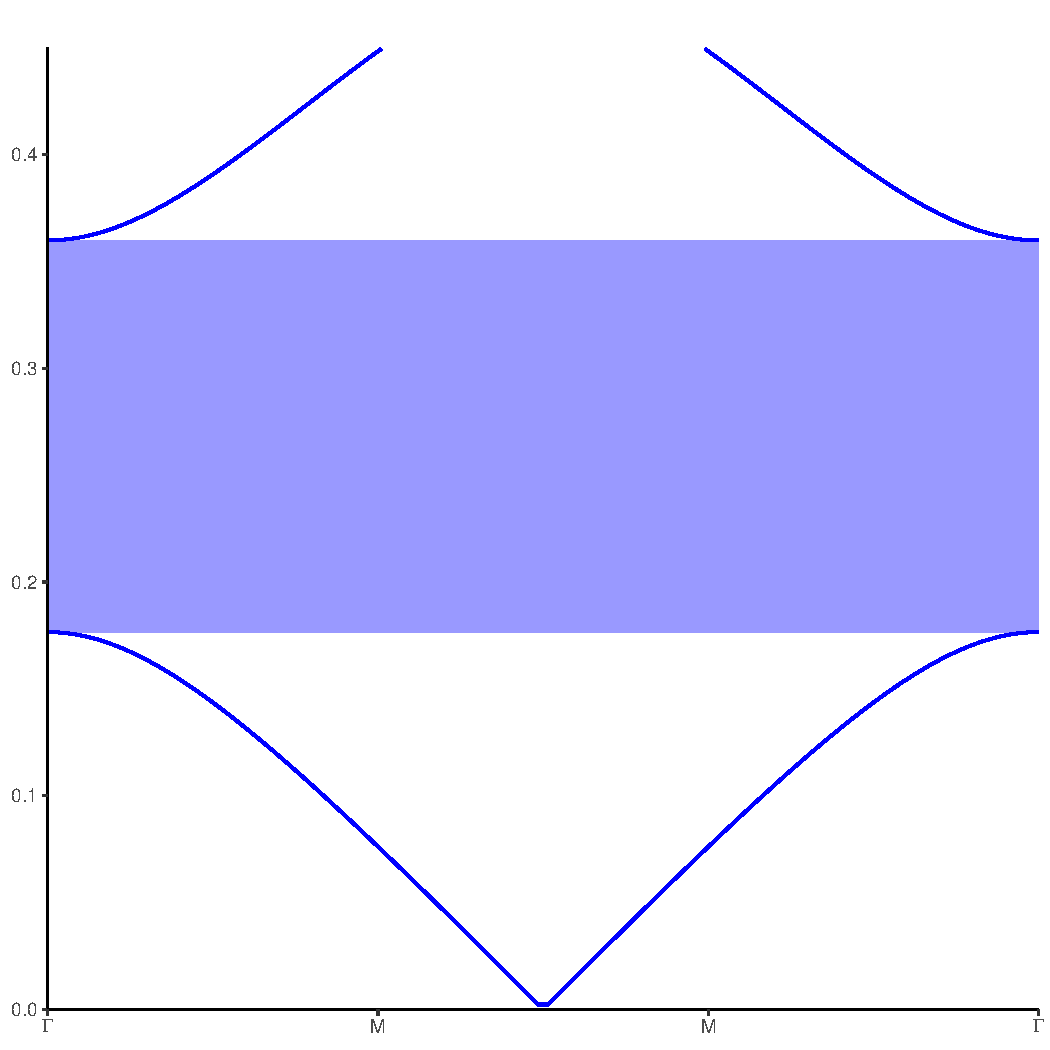
\includegraphics[width = 1.0\linewidth]{./images/1d_crystal_gap.pdf}
	\caption{Fotonički frekvencijski raspor u jednodimenzionalnoj strukturi}
	\label{fig:1d_band_diagram}
\end{figure}

Rezultat \ref{eq:rayleighE} kaže da će prvi pojas većinu svoje energije
pohraniti unutar sredstva veće permitivnosti. U slučaju modela koji se
promatra, to je sredstvo čija je relativna permitivnosti 12. Taj pojas
u nastavku će se nazivati \emph{dielektrični pojas}. Pojas iznad raspora mora
osigurati jednaku simetriju kao i struktura, ali pored toga, mora osigurati i
ortogonalnost u odnosu na dielektrični pojas. Drugim riječima, pojas iznad
raspora mora imati jednak period jer njega diktira struktura, ali ne smije svoju
energiju pohraniti unutar istog sredstva. Rješenje koje se nameće je da pojas
iznad raspora energiju pohrani u sredstvu manje permitivnosti i k tome zadrži
isti period. Pojas iznad dielektričnog, u nastavku će se nazivati \emph{zračni
pojas} jer će njegova energija biti pohranjena u sredstvu manje permitivnosti,
a ono je najčešće zrak.

U kristalu su u ovom trenutku 2 vala s istim periodom, energija jednog je
većinom pohranjena u dielektriku, a energija drugog je većinom pohranjena
u zraku. Ovi valovi moraju ``vidjeti'' različite prosječne indekse loma.
Dielektrični pojas propagira s većim indeksom loma budući da većinu svoje energije
pohranjuje upravo u sredstvu veće permitivnosti, a s druge strane, zračni pojas
propagira s manjim prosječnim indeksom loma budući da svoju energiju
većinom pohranjuje u sredstvu manje permitivnosti. Sve to, navodi na zaključak
da pojasevi moraju imati različite frekvencije. Frekvencijski raspor u ovom
slučaju je upravo ta razlika frekvencija koja nastaje zbog različitog prosječnog
indeksa loma.

\FloatBarrier
Unutar fotoničkog frekvencijskog raspora nema propagacije vala. Val čija se
frekvencija nalazi unutar frekvencijskog raspora naziva je evanescentni val i
njegova amplituda eksponencijalno teži u 0. Evanescentni val ima kompleksni valni
vektor ${\bm{\beta}} + j \kappa$ gdje je $\kappa$ faktor prigušenja.

\begin{equation} \label{eq:evan}
	\mathbf{E}(\mathbf{r}) =
	\mathbf{A}_{\bm{\beta}}(\mathbf{r}) \cdot
		e^{j ({\bm{\beta}} + j \kappa) \cdot \mathbf{r}} =
	\mathbf{A}_{\bm{\beta}}(\mathbf{r}) \cdot
		e^{j {\bm{\beta}} \cdot \mathbf{r}} e^{-\kappa \cdot \mathbf{r}}
\end{equation}


\section{Kvadratna rešetka dielektričnih stupića}

U ovom primjeru, fotonički kristal građen je od dielektričnih stupića
postavljenih tako da gledano iz smjera z osi izgledaju kao slika
\ref{fig:square_lattice}

\begin{figure}[ht]
	\centering
	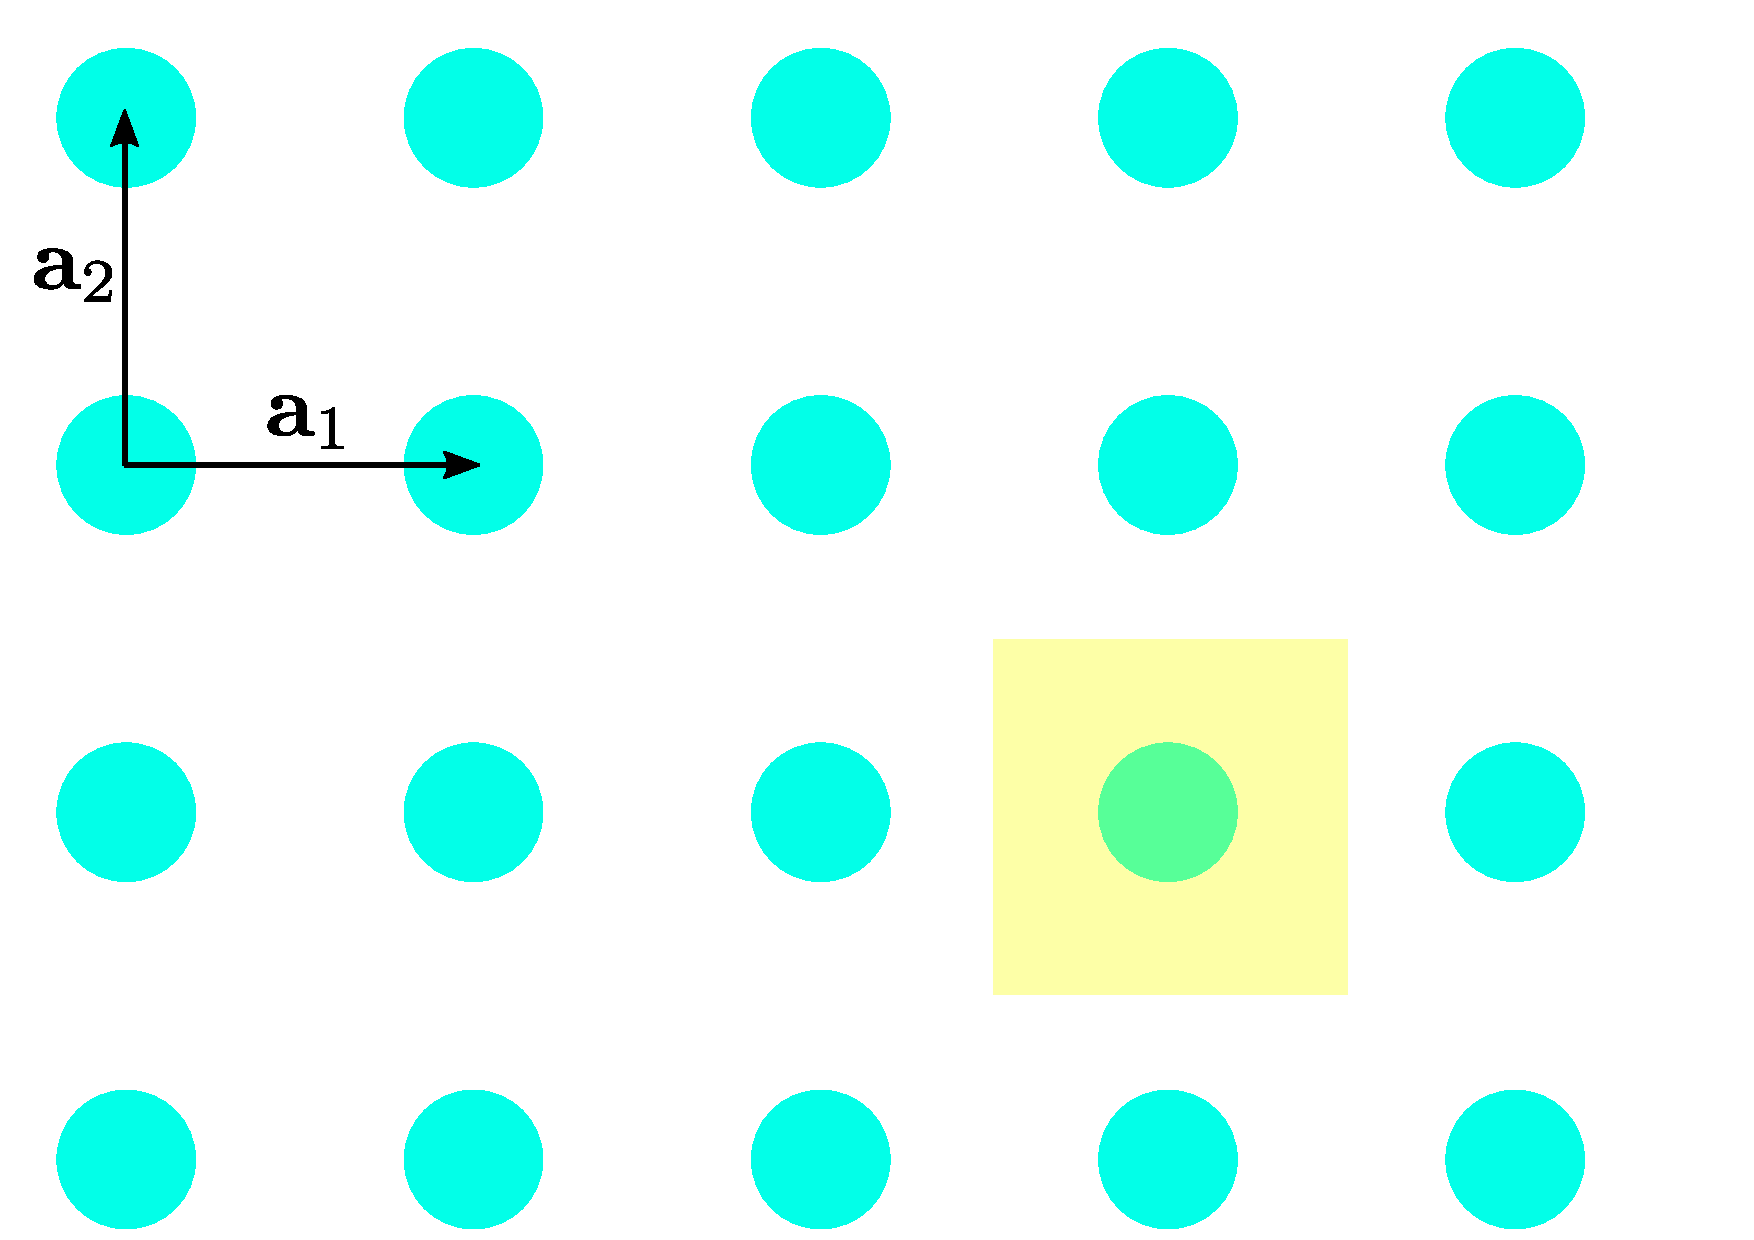
\includegraphics[width = 1.0\linewidth]{./images/square_lattice.pdf}
	\caption{Kvadratna rešetka s ucrtanim baznim vektorima i Weigner-Seintzovom
	ćelijom. Polumjer stupića u ovom modelu kristala iznosi ${0.2 a}$, odnosno
	promjer stupića zauzima 40\% duljine jedinične čelije.}
	\label{fig:square_lattice}
\end{figure}

Bazni vektori rešetke su vektori ${\mathbf{a}_1 = a \, \mathbf{i}}$ i
${\mathbf{a}_2= a \, \mathbf{j}}$, a Weigner-Seintzova ćelija označena je
desno žutom bojom. Bazni vektori recipročne rešetke su
${\mathbf{b}_1 = 2 \pi/a \, \mathbf{i}}$ i
${\mathbf{b}_2 = 2 \pi/a \, \mathbf{j}}$, a prva Brillouinova zona prikazana
je na disperzijskom dijagramu \ref{fig:square_band_diagram}.

\begin{figure}[ht]
	\centering
	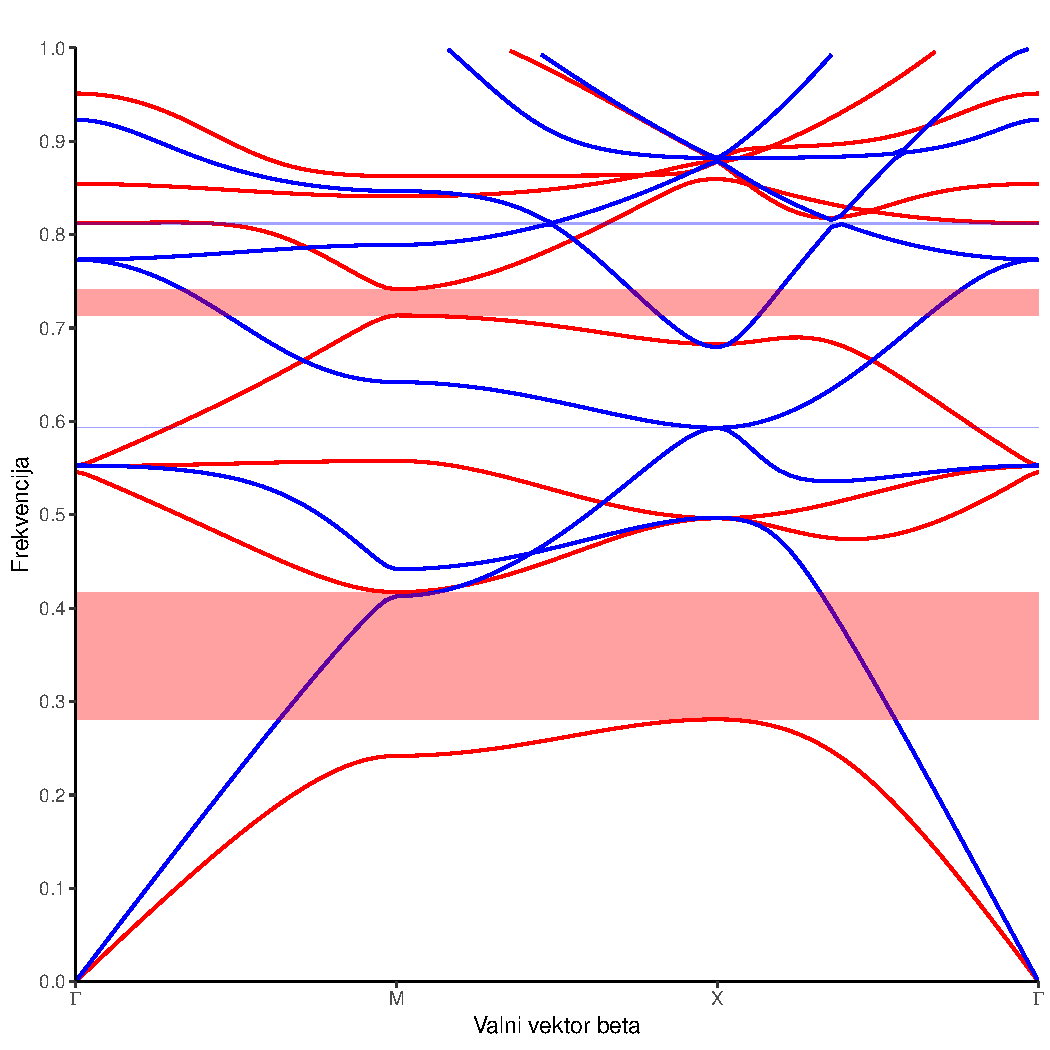
\includegraphics[width = 1.0\linewidth]{./images/square.pdf}
	\caption{Disperzijski dijagram za kvadratnu rešetku koju sačinjavaju
	dielektrični stupići. Frekvencijski raspor prisutan je samo za TM mod. Na
	dijagramu je označena i prva Brillouinova zona s pripadnim oznakama na x osi.}
	\label{fig:square_band_diagram}
\end{figure}

\FloatBarrier

\section{Trokutasta rešetka dielektričnih stupića} \label{sec:triangle}

U ovom primjeru, fotonički kristal građen je od dielektričnih stupića
postavljenih tako da gledano iz smjera z osi izgledaju kao
slika \ref{fig:triangular_lattice}

\begin{figure}[ht]
	\centering
	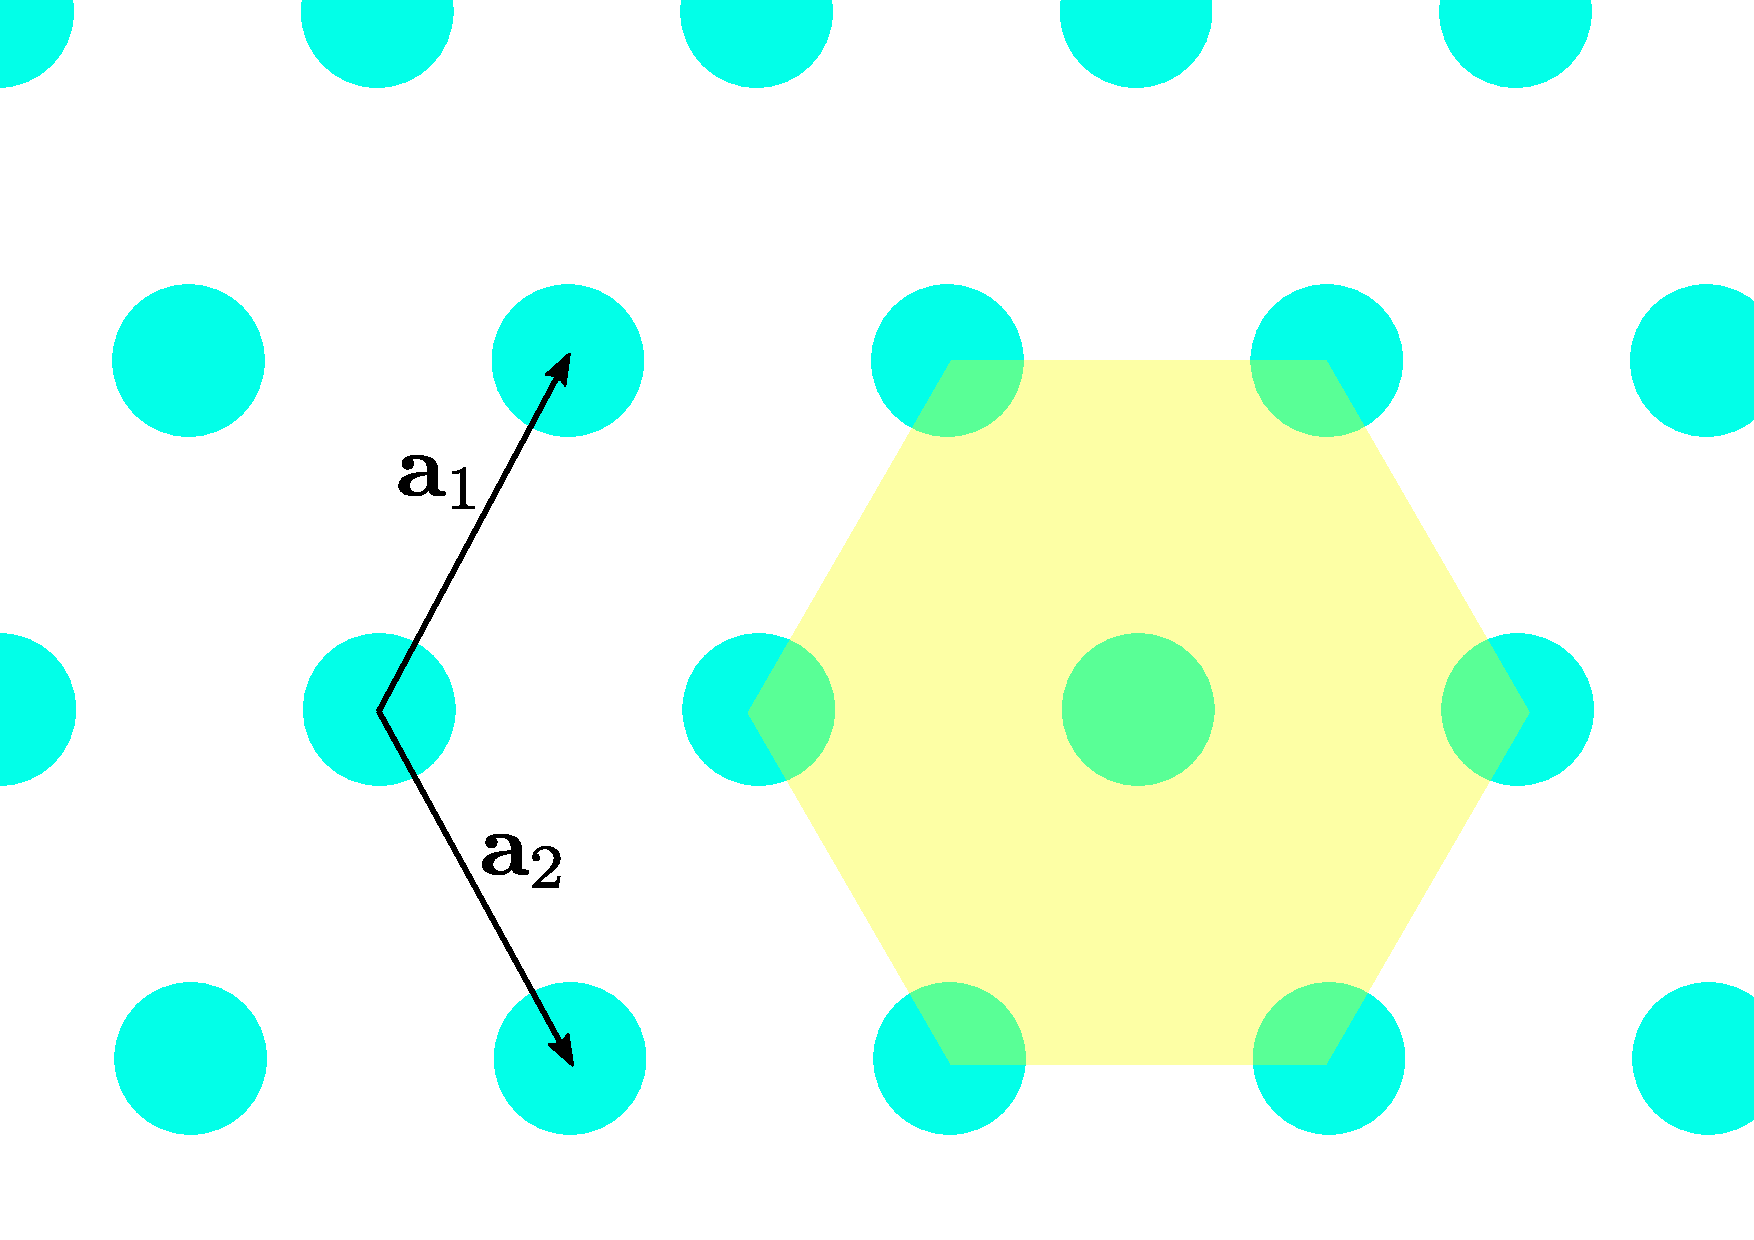
\includegraphics[width = 1.0\linewidth]{./images/triangular_lattice.pdf}
	\caption{Trokutasta rešetka s ucrtanim baznim vektorima i Weigner-Seintzovom
	ćelijom. Polumjer stupića u ovom modela kristala iznosi ${0.2 a}$, odnosno
	promjer stupića zauzima 40\% duljine jedinične ćelije.}
	\label{fig:triangular_lattice}
\end{figure}

Bazni vektori rešetke su vektori
${\mathbf{a}_1 = a/2 ( \, \mathbf{i} + \sqrt{3} \, \mathbf{j})}$ i
${\mathbf{a}_2 = a/2 ( \, \mathbf{i} - \sqrt{3} \, \mathbf{j})}$.
a Weigner-Seintzova ćelija označena je desno žutom bojom.
Bazni vektori recipročne rešetke su
${\mathbf{b}_1 = 2 \pi/a( \, \mathbf{i} + 1/\sqrt{3} \, \mathbf{j})}$ i
${\mathbf{b}_2 = 2 \pi/a( \, \mathbf{i} - 1/\sqrt{3} \, \mathbf{j})}$,
a prva Brillouinova zona prikazana je na disperzijskom dijagramu
\ref{fig:triangular_band_diagram}.

\begin{figure}[ht]
	\centering
	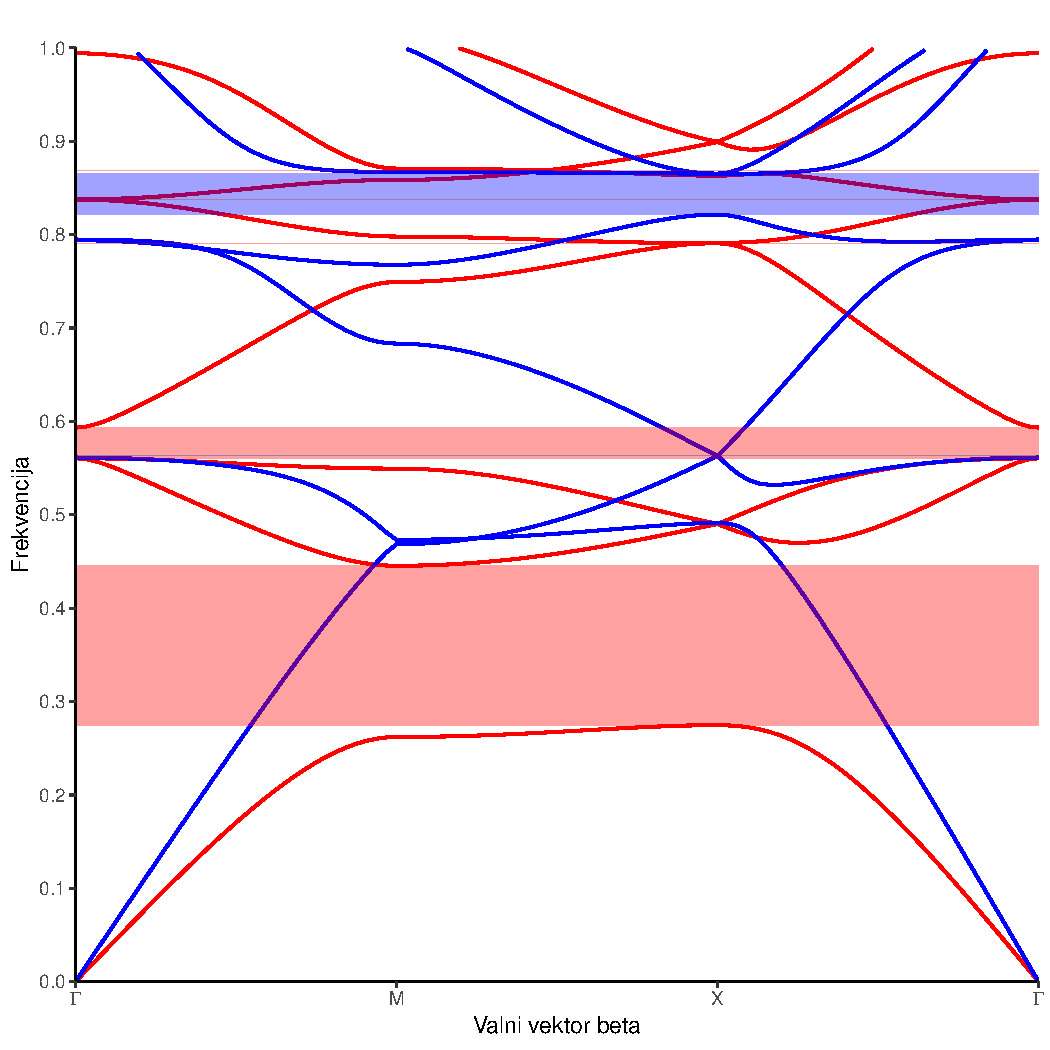
\includegraphics[width = 1.0\linewidth]{./images/triangular.pdf}
	\caption{Disperzijski dijagram za trokutastu rešetku koju sačinjavaju
	dielektrični stupići. Frekvencijski raspor prisutan je i za TE mod i za TM
	mod. Na dijagramu je označena i prva Brillouinova zona s pripadnim oznakama.}
	\label{fig:triangular_band_diagram}
\end{figure}

\FloatBarrier

\section {Trokutasta rešetka za potpuni frekvencijski raspor}

U ovom primjeru fotonički kristal građen je od zračnih rupa u dielektričnom
materijalu. Gledano iz smjera z osi, kristal izgleda kao na slici
\ref{fig:triangular_lattice_holes}.

\begin{figure}[ht]
	\centering
	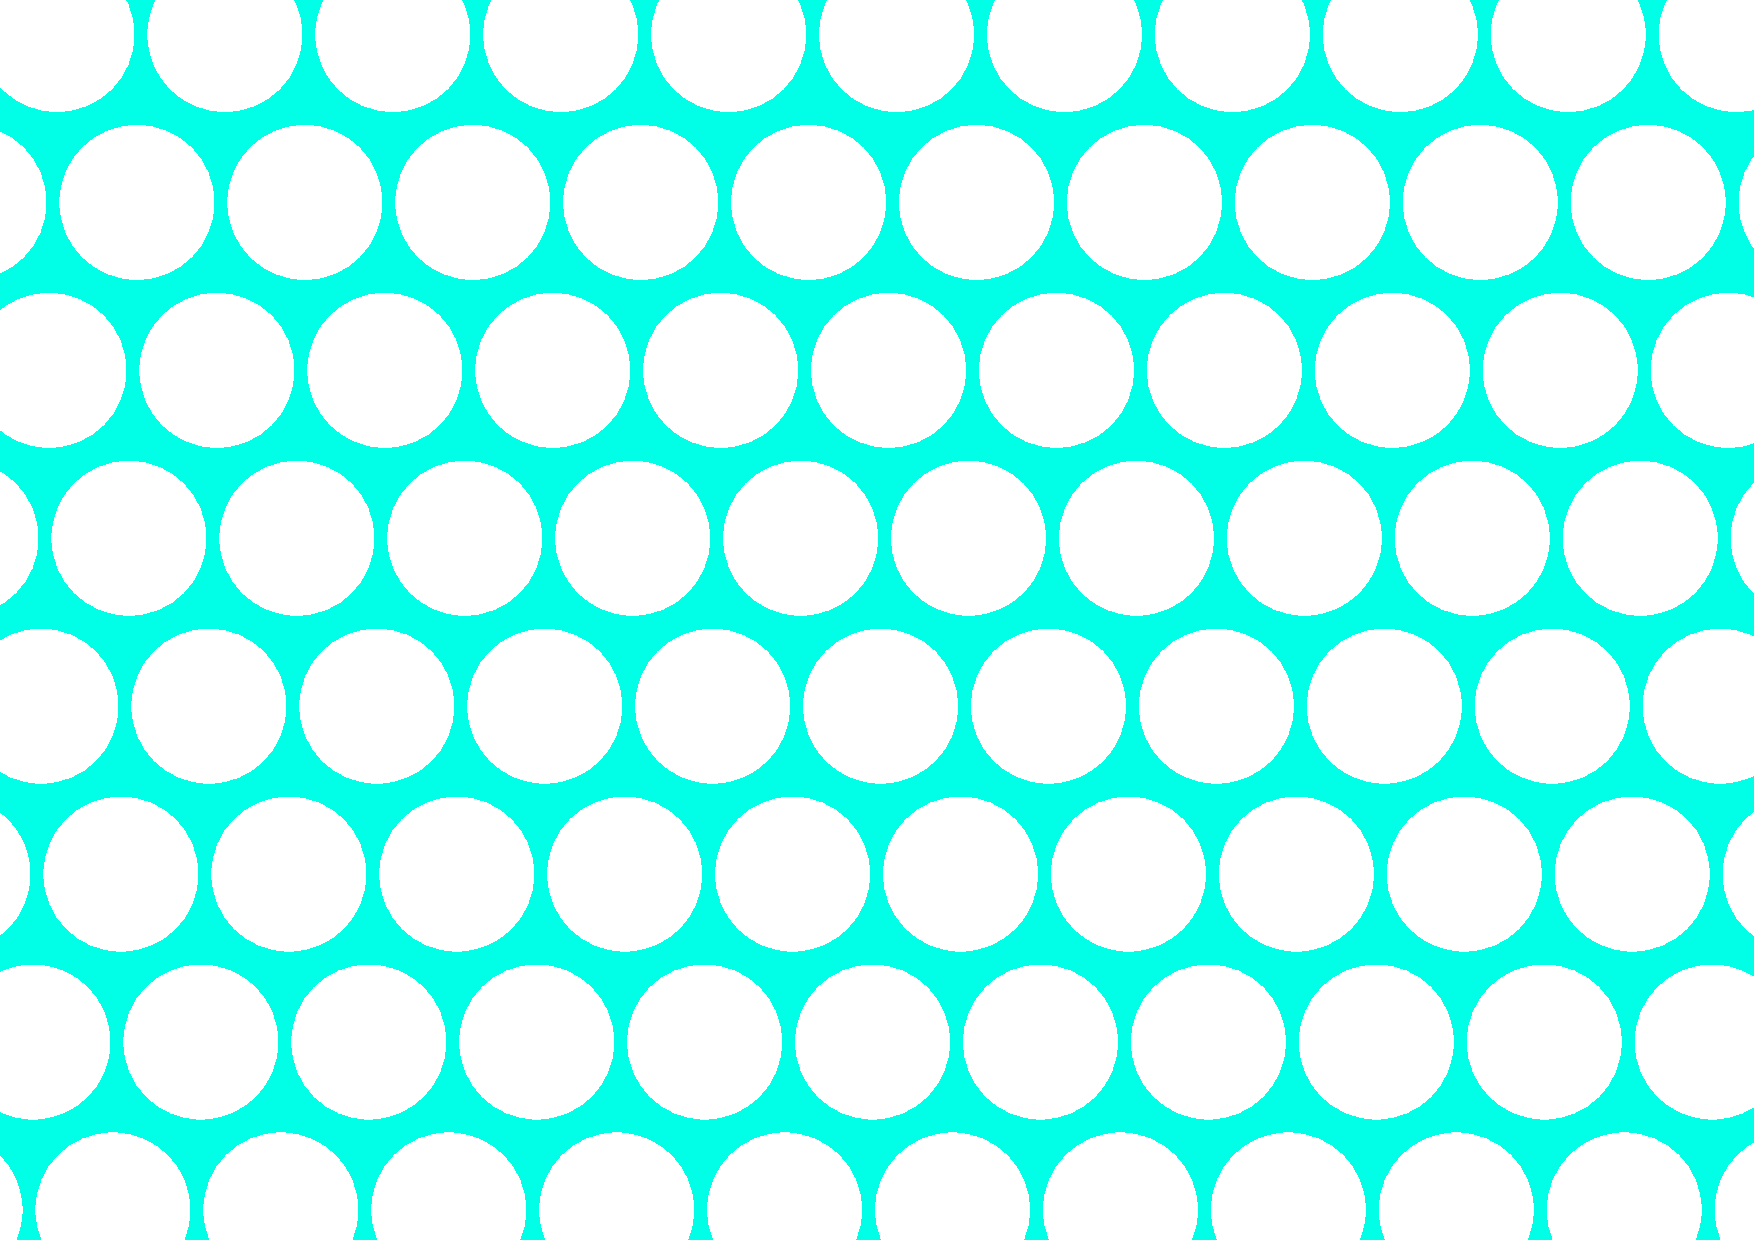
\includegraphics[width = 1.0\linewidth]{./images/triangular_lattice_holes.pdf}
	\caption{Na slici nisu ucrtane Brillouinova zona i primitivni vektori rešetke
	jer su u odnosu na sliku \ref{fig:triangular_lattice} samo drugačijeg iznosa.
	Polumjer stupića u ovoj rešetci iznosi ${0.45 \, a}$, odnosno promjer stupića
	iznosit će 90 \% duljine jedinične ćelije.}
	\label{fig:triangular_lattice_holes}
\end{figure}

Na disperzijskom dijagramu \ref{fig:triangular_full_band} u ovom slučaju postoji
potpuni frekvencijski raspor.

\begin{figure}[ht]
	\centering
	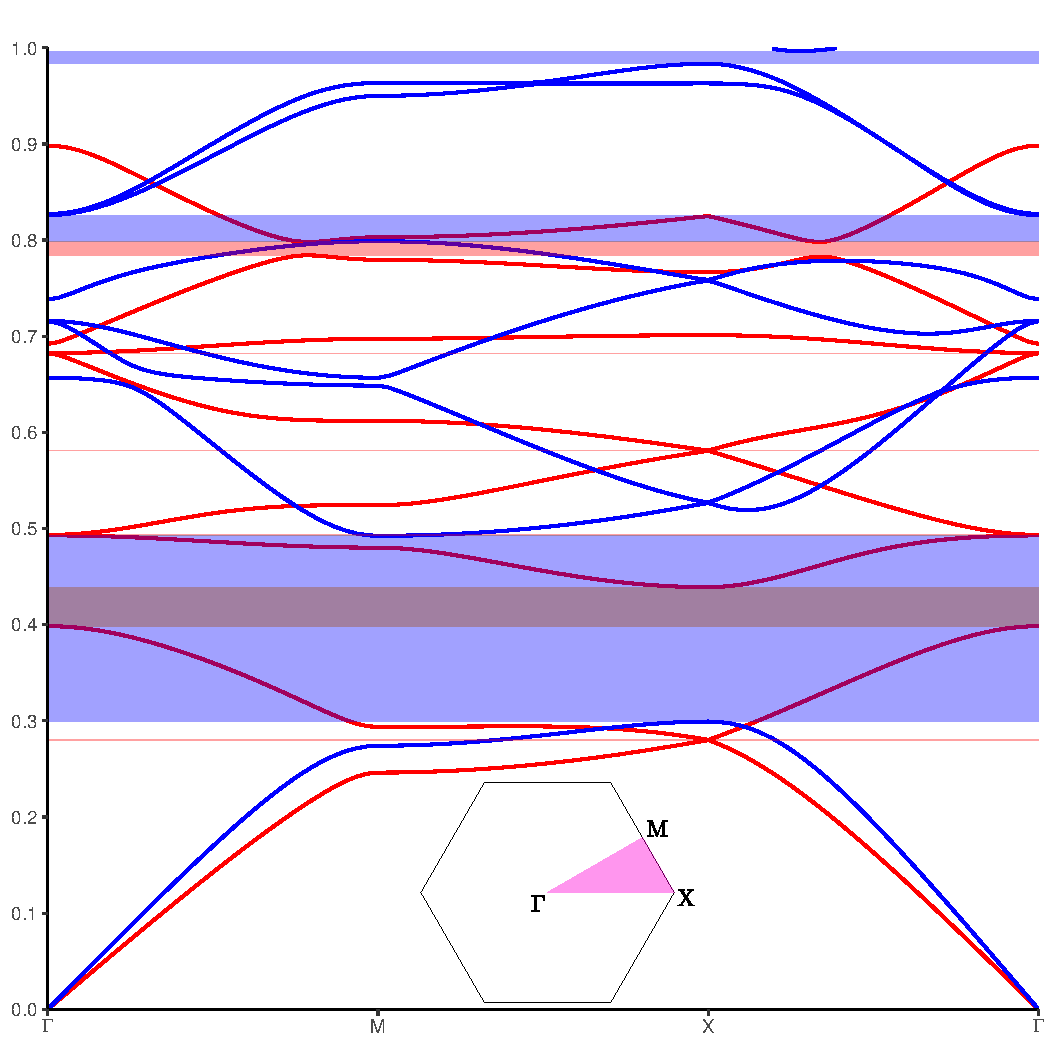
\includegraphics[width = 1.0\linewidth]{./images/triangular_holes.pdf}
	\caption{Disperzijski dijagram za fotonički kristal kojeg sačinjavaju rupe
	u dielektričnom materijalu. Plavim pravokutnikom je označen frekvencijski
	raspor za TE, a crvenim za TM mod. Na ovoj slici se unutar
	plavog raspora nalazi crveni, odnosno unutar raspora za TE mod, nalazi se
	raspor za TM mod. Ta pojava naziva se potpuni frekvencijski raspor (engl.
	\textit{full band-gap}). Za frekvencije unutar raspora nema modova koji
	mogu propagirati kroz strukturu. Na dijagramu je označena i prva Brillouinova
	zona s pripadnim oznakama.}
	\label{fig:triangular_full_band}
\end{figure}

\FloatBarrier

Val čija je frekvencija unutar frekvencijskog raspora naziva se evanescentan.
Njegova amplituda trnut će eksponencijalno. U ovu strukturu je uz unošenje
defekata moguće lokalizirati harmonik. Defekt je strogo gledano nepravilnost
koja će na ovaj ili onaj način narušiti simetriju kristala.

\chapter{Optimizacija širine potpunog frekvencijskog raspora trokutaste rešetke}

\chapter{Zaključak}
Zaključak.

\bibliographystyle{unsrt}
\bibliography{literatura}
\nocite{*}

\end{document}
